%% This paper is distributed through its repository,
%% https://github.com/urdvr/superperm-coeff2, which also contains a complete Lean 4
%% formalization of every numbered display and named result (Coeff2/Statements.lean,
%% one theorem per paper item; AxiomCheck.lean is the executable axiom audit).  The
%% paper text itself is self-contained and classical.
\documentclass[11pt]{article}

\usepackage[margin=1.05in]{geometry}
\usepackage{amsmath,amssymb,amsthm}
\usepackage{mathtools}
\PassOptionsToPackage{hyphens}{url}
\usepackage[hidelinks]{hyperref}
\usepackage{tikz}
\usetikzlibrary{decorations.pathreplacing}

\newtheorem{theorem}{Theorem}
\newtheorem{lemma}[theorem]{Lemma}
\newtheorem{proposition}[theorem]{Proposition}
\newtheorem{corollary}[theorem]{Corollary}
\newtheorem{definition}[theorem]{Definition}
\newtheorem{remark}[theorem]{Remark}

\DeclareMathOperator{\wt}{wt}
\DeclareMathOperator{\len}{len}
\newcommand{\HPV}{\mathrm{HPV}}

\title{A Coefficient-Two Additive Improvement to the HPV Lower Bound for Superpermutations}
\author{Uku Raudvere\thanks{This is an AI-derived result: the proofs were produced by AI
systems under the author's direction --- see the provenance statement before the
bibliography.}}
\date{}

\begin{document}
\maketitle

\begin{abstract}
Let \(S(n)\) be the minimum length of a word on \([n]\) containing every permutation of \([n]\) as a
factor.  The lower bound of Anonymous--Houston--Pantone--Vatter (HPV) is
\[
  S(n)\ge \HPV(n):=n!+(n-1)!+(n-2)!+n-3.
\]
We prove that for all \(n\ge 5\),
\[
  S(n)\ \ge\ n!+(n-1)!+(n-2)!+n-3+\Bigl\lceil\tfrac{(n-3)!-1}{2n-1}\Bigr\rceil .
\]
The bound arises by solving a linear criterion in closed form: for every \(k\ge 0\) satisfying
\((2k(n-1)+1)(n-2)+k(n-1)<(n-2)!+k\) we show \(S(n)\ge\HPV(n)+k+1\), and the ceiling above is
exactly the largest value of \(k+1\) that the criterion admits.  The \(k=0\) instance already
gives \(S(n)\ge\HPV(n)+1\) for all \(n\ge5\) --- an improvement announced by Houston and
reported in the Engen--Vatter survey \cite{EV}, for which, to the author's knowledge, no
proof had been published --- and
for \(n\ge7\) the bound strictly exceeds \(\HPV(n)+1\) and grows factorially: in particular
\(S(6)\ge 868\), \(S(7)\ge 5886\), and uniformly \(S(n)\ge\HPV(n)+\lceil(n-4)!/3\rceil\)
for all \(n\ge5\).  At
\(n=5\) the bound reads \(S(5)\ge 153\), which equals the known exact value.  To the author's
knowledge (as of July 2026) this is the first strengthening of the HPV bound whose gain grows
factorially with \(n\).
The proof follows the HPV overlap-graph method.  We retain their parameters \(p,c,v\), rewrite the
HPV inequality as an exact excess identity, and then count the \emph{breaks} --- the deviations
from a canonical successor --- in the list of entered marked \(2\)-loops, ordered by first entry.
Each break either meets an edge of positive defect or is charged to a rotation orbit shared by
two of the loops; the new point is that a slot receiving two charges also forces two consecutive
breaks, which shortens one canonical block by \(n-3\).  This converts the
coefficient \(3\) that the charge count alone would give into the coefficient \(2\) used below.
\end{abstract}

\section{Introduction}

A word over the alphabet \([n]=\{1,\ldots,n\}\) is an \emph{\(n\)-superpermutation} if it contains
every permutation of \([n]\) as a factor (a block of \(n\) consecutive symbols).  Let \(S(n)\)
denote the minimum length of an \(n\)-superpermutation.  The exact values
\[
  S(1)=1,\quad S(2)=3,\quad S(3)=9,\quad S(4)=33,\quad S(5)=153
\]
are known (see also \cite{J2013}), the last by Chaffin's verification \cite{JohnstonBlog,OEIS}; already \(S(6)\) is open: the
best bounds are \(868\le S(6)\le 872\), where the lower bound --- announced by Houston, see
below --- is given a self-contained proof in Theorem \ref{thm:intromain}.  For a
long time the natural construction of length \(\sum_{k=1}^{n}k!\) was conjectured optimal
\cite{AT}; Houston \cite{Houston} disproved this at \(n=6\) with a superpermutation of length
\(872\).  On the lower-bound side, the breakthrough is the note of an anonymous contributor with
Houston, Pantone, and Vatter \cite{HPV}, which proves
\[
  S(n)\ \ge\ \HPV(n)\ :=\ n!+(n-1)!+(n-2)!+n-3 .
\]
Houston subsequently showed, in the Superpermutators group (the online collaboration around
this problem), that this bound can be increased by
\(1\); the improvement is reported in the Engen--Vatter survey \cite{EV} as, together with
Egan's construction below, the best general result to date, but, to the author's knowledge
(as of July 2026), no proof of it has been
published.  Theorem \ref{thm:intromain} below proves \(S(n)\ge\HPV(n)+1\) for all
\(n\ge 5\) (the \(k=0\) instance of the criterion).
In the other direction, Egan \cite{Egan} constructed, for every \(n\ge 7\), superpermutations of
length
\[
  n!+(n-1)!+(n-2)!+(n-3)!+n-3\ =\ \HPV(n)+(n-3)!,
\]
so the gap between these two bounds is exactly \((n-3)!\).

This paper strengthens the HPV lower bound by an amount that grows factorially with \(n\).

\begin{theorem}[main theorem; proved as Theorem \ref{thm:solved}]
\label{thm:intromain}
For all \(n\ge 5\),
\[
  S(n)\ \ge\ \HPV(n)+\Bigl\lceil\frac{(n-3)!-1}{2n-1}\Bigr\rceil .
\]
The ceiling is exactly what the criterion is worth: for \(k\ge 0\), the
\emph{criterion}
\[
  \bigl(2k(n-1)+1\bigr)(n-2)+k(n-1)<(n-2)!+k
\]
implies \(S(n)\ge \HPV(n)+k+1\), and the criterion holds if and only if
\(k(2n-1)<(n-3)!-1\), i.e.\ if and only if \(k<\bigl\lceil((n-3)!-1)/(2n-1)\bigr\rceil\)
(Lemma \ref{lem:solve}).  In particular
\begin{gather*}
  S(5)\ge\HPV(5)+1=153,\qquad
  S(6)\ge\HPV(6)+1=868,\\
  S(7)\ge\HPV(7)+2=5886,\qquad
  S(8)\ge\HPV(8)+8,\\
  S(9)\ge\HPV(9)+43,\qquad
  S(10)\ge\HPV(10)+266,\qquad
  S(11)\ge\HPV(11)+1920,
\end{gather*}
and, uniformly over the whole range, for all \(n\ge5\),
\[
  S(n)\ \ge\ \HPV(n)+\Bigl\lceil\frac{(n-4)!}{3}\Bigr\rceil .
\]
\end{theorem}

\noindent
(The point values are Corollaries \ref{cor:pointvalues} and \ref{cor:words}; the
factorial form is Corollary \ref{cor:third}.)
Numerically, the first cases read as follows.  The upper bounds are: at \(n=6\), Houston's
\(872\) \cite{Houston}; at \(n=7\), the record \(5906\) of Egan and Houston (February 2019,
refining Coanda's \(5907\); see \cite{Egan,EV}), two below the general construction's \(5908\);
for \(n\ge 8\), Egan's construction \cite{Egan}.
\[
\begin{array}{c|c|c|c}
n & \HPV(n) & \text{this paper} & \text{best upper bound}\\ \hline
5 & 152 & 153 & 153\ (=S(5))\\
6 & 867 & 868 & 872\\
7 & 5884 & 5886 & 5906\\
8 & 46085 & 46093 & 46205\\
9 & 408246 & 408289 & 408966\\
10 & 4032007 & 4032273 & 4037047\\
11 & 43908488 & 43910408 & 43948808
\end{array}
\]
The improvement is \(\lceil((n-3)!-1)/(2n-1)\rceil\sim(n-3)!/(2n)\), of order \((n-4)!\),
against a total gap of \((n-3)!\).  (The displayed factorial form is a weaker but more memorable consequence, with an
elementary certificate, Lemma \ref{lem:third}; it is dominated by the ceiling, with
equality at \(5\le n\le 8\).)

At the bottom of the range the criterion is exhausted: at \(n=6\) its inequality holds at
\(k=0\) and fails at \(k=1\), so this accounting yields nothing beyond \(868\); at \(n=5\)
it likewise caps at \(k=0\), and the resulting bound \(S(5)\ge 153\) equals the known exact
value.  (At \(n=5\) the \(k=0\) instance of the criterion rules out precisely the covering walks of
length exactly \(\HPV(5)\); consistently, superpermutations of length \(\HPV(5)+1\)
exist.)  Below
\(n=5\) the statement is void: \(S(n)\) is classical for \(n\le 4\).

\subsection*{Method}

The proof takes place in the HPV weighted overlap graph and keeps their three parameters: the
number \(p\) of distinct permutations visited, the number \(c\) of completed cyclic (rotation)
classes, and the number \(v\) of entered marked \(2\)-loops.  Section 3 recalls the HPV
monovariant \(\wt(W)\ge p+c+v-2\) and rewrites it as an exact excess identity
\(\len(W)=\HPV(n)+e+r+\ell\).  Section 4 orders the entered marked \(2\)-loops by first entry and
compares consecutive entries with a canonical successor map of period \(n-2\); the positions where
the walk deviates from the successor are \emph{breaks}, and \(v\le(|A|+1)(n-2)\) for \(|A|\)
breaks.  Section 5 is the heart of the paper: a completely local analysis of a break window,
which shows that every break not accounted for by a positive-defect edge deposits a \emph{charge}
on a shared rotation orbit, and that the charges are almost injective --- each incident slot
receives at most two, and a slot receiving two forces two \emph{consecutive} breaks whose
intervening block has length \(1\) instead of \(n-2\); the double-charged slots, the a priori
loss in the charge count, are thus compensated up to a residual of one break per slot by the
\(n-3\) saving of their short blocks.  Section 6 assembles the counts: the residual is absorbed
by the lower-order \(k(n-1)\) term of the criterion, the resulting inequality carries the
coefficient \(2\) of the title, and solving the criterion, which is linear in \(k\), gives the
ceiling.  Section 7 verifies the closed-form arithmetic.

The presentation is self-contained: we use the objects of \cite{HPV} --- the overlap graph,
the marked \(2\)-loops, and the monovariant --- but every property of them that the argument
needs is proved here from scratch.

\subsection*{Availability}

This paper is distributed through its repository at
\url{https://github.com/urdvr/superperm-coeff2}, which also contains a complete
machine-checked formalization (in Lean 4, over mathlib) of every numbered display and
every named result of this paper, one theorem per item in paper order, together with
build instructions and an executable axiom audit.  The paper is distributed under the
Creative Commons Attribution 4.0 International license (CC BY 4.0); the formalization
is released under the Apache License 2.0.

\section{The graph}

We use the weighted directed graph from the HPV proof \cite{HPV}.  Its vertices are the \(n!\) permutations of
\([n]\); write \(S_n\) for their set.  If \(\pi,\sigma\in S_n\), the edge weight
\[
  \wt(\pi,\sigma)
\]
is the least number of symbols that must be appended after an occurrence of \(\pi\) so that the last
\(n\) symbols become \(\sigma\).  Equivalently,
\[
  \wt(\pi,\sigma)=\min\{d:1\le d\le n,\;
    \pi_{d+1}\cdots \pi_n=\sigma_1\cdots\sigma_{n-d}\}.
\]
It is useful to spell out the proper-edge reduction, because properness is used later in the local
word calculations.  Suppose an edge \(\pi\to\sigma\) has weight \(d\), so the word obtained by
appending the final \(d\) symbols of \(\sigma\) to \(\pi\) is
\[
  \pi_1\cdots\pi_n\sigma_{n-d+1}\cdots\sigma_n .
\]
The edge is improper if one of the intermediate length-\(n\) windows, at an offset
\(1\le h<d\), is already a permutation.  Equivalently, if
\[
  \sigma=s_{d+1}\cdots s_n t_1\cdots t_d
\]
is written from \(\pi=s_1\cdots s_n\), then the edge is proper precisely when
\[
  \{t_1,\ldots,t_h\}\ne\{s_1,\ldots,s_h\}\qquad(1\le h<d). \tag{prop}
\]
If an edge is improper, splitting at the first intermediate permutation writes it as two overlap
edges whose weights sum to at most the original weight; repeating this process expresses it as a
path of proper edges of total weight at most the original.  Hence deleting improper edges does not
increase the minimum length of a covering walk.  Every superpermutation gives a covering walk in this proper overlap
graph of length at most the word length: record the permutation windows from left to right and
replace any improper overlap edge by its proper-edge refinement.

For a walk \(W=(\pi_1,\ldots,\pi_m)\) in the proper overlap graph (a sequence of vertices with
consecutive vertices joined by proper edges), write
\[
  \wt(W)=\sum_{i=1}^{m-1}\wt(\pi_i,\pi_{i+1}),\qquad
  \len(W)=n+\wt(W).
\]
A walk is covering if it visits every permutation at least once.  Let
\[
  \Lambda(n)=\min\{\len(W):W\text{ is a covering walk}\}.
\]
Since every \(n\)-superpermutation gives a covering walk no longer than the word itself,
\[
  \Lambda(n)\le S(n).
\]
It is enough to prove the lower bound for \(\Lambda(n)\).  In fact the reduction is exact,
so nothing is lost in passing to walks.

\begin{proposition}[The walk model is exact]\label{prop:exactmodel}
\(\Lambda(n)=S(n)\) for all \(n\ge1\).
\end{proposition}

\begin{proof}
For the direction \(S(n)\le\Lambda(n)\), let \(W=(\pi_1,\ldots,\pi_m)\) be a covering walk,
put \(w_i=\wt(\pi_i,\pi_{i+1})\), and write \(\pi[1..d]\) for the first \(d\) symbols of a
permutation \(\pi\).  Form the word
\[
  \pi_1[1..w_1]\;\pi_2[1..w_2]\;\cdots\;\pi_{m-1}[1..w_{m-1}]\;\pi_m .
\]
Its length is exactly \(w_1+\cdots+w_{m-1}+n=\wt(W)+n=\len(W)\), and by the defining overlap
identity (the last \(n-w_i\) symbols of \(\pi_i\) are the first \(n-w_i\) symbols of
\(\pi_{i+1}\)) the word of each visited vertex occurs in it as a factor at that vertex's
position; coverage makes it an \(n\)-superpermutation.
\end{proof}

Everything below is therefore a statement about \(S(n)\) itself;
in the proofs we work with \(\Lambda(n)\) and use only the direction \(\Lambda(n)\le S(n)\).

\section{The HPV accounting}

Throughout Sections 3--5 we assume \(n\ge 4\).  (The objects below degenerate at very
small \(n\): at \(n=3\), for instance, the word \(r\) of Section 4 is empty and the
canonical corner exit has weight \(2\) rather than \(3\), and at \(n=2\) the weight-\(2\)
door coincides with the rotation.  Everything from Section 6 onward concerns \(n\ge 5\),
so no generality is lost.)

The weight-\(1\) edge out of
\[
  \pi=\pi_1\pi_2\cdots\pi_n
\]
is the cyclic rotation
\[
  \pi_2\pi_3\cdots\pi_n\pi_1.
\]
The cyclic classes are the orbits of this rotation; there are \((n-1)!\) of them, each of size \(n\).

The weight-\(2\) door out of \(\pi\) --- the unique proper weight-\(2\) edge (Lemma
\ref{lem:localtight}); it always leaves the current cyclic class, since staying would force
\(\pi_2=\pi_3\) (compare the cyclic successor of \(\pi_1\) in the two words) --- is
\[
  \pi_3\pi_4\cdots\pi_n\pi_2\pi_1.
\]
Following rotations and these weight-\(2\) doors gives the HPV \(2\)-loops.  We use the following
explicit form.  A marked \(2\)-loop is a pair
\[
  L=(\alpha,K),
\]
where \(\alpha\in[n]\) (the \emph{marker}) and \(K\) is a cyclic class of words using the
\(n-1\) symbols in \([n]\setminus\{\alpha\}\).  Its vertex set is
\[
  V(L)=\{\sigma\in S_n:\operatorname{del}_\alpha(\sigma)\in K\},
\]
where \(\operatorname{del}_\alpha(\sigma)\) denotes the word obtained by deleting \(\alpha\) from \(\sigma\).
Deleting \(\alpha\) from \(\rho(\sigma)\) yields a cyclic rotation of \(\operatorname{del}_\alpha(\sigma)\),
and \(K\) is a cyclic class; hence \(V(L)\) is closed under cyclic rotation.
Thus the loop generated by \(\pi_1\cdots\pi_n\) is
\[
  \bigl(\pi_n,\,[\pi_1\cdots\pi_{n-1}]\bigr).
\]
Throughout, \(L(\sigma)\) denotes the marked \(2\)-loop generated by \(\sigma\).
Each marked \(2\)-loop contains \(n(n-1)\) permutations, and there are \(n(n-2)!\) such loops.  A
single permutation lies in one marked loop for each possible deleted symbol.

We now fix the dynamic convention used throughout the proof.  For a walk
\[
  W=(\pi_1,\ldots,\pi_m),
\]
let \(H_t\) be the marked \(2\)-loop being followed at time \(t\).  Define
\[
  H_1=L(\pi_1),
\]
and, for \(t>1\),
\[
  H_t=
  \begin{cases}
  L(\pi_t),&\text{if }\wt(\pi_{t-1},\pi_t)\ge2,\\
  H_{t-1},&\text{if }\wt(\pi_{t-1},\pi_t)=1.
  \end{cases}
\]
Thus a weight-\(1\) rotation keeps the active marked loop, while a nonrotation edge activates the
marked loop generated by its landing vertex.  A marked \(2\)-loop is \emph{entered} if it occurs
among the \(H_t\), and is \emph{first entered} at the least such time.  A later nonrotation edge may
activate an already entered loop; such a later activation does not increase \(v\).  With this
convention every visited permutation lies in the active marked loop \(H_t\) --- a nonrotation
arrival activates the loop generated by its landing vertex, which contains it, and a weight-\(1\)
rotation preserves membership because \(V(L)\) is closed under rotation --- and therefore lies in
at least one entered marked \(2\)-loop.  A covering walk therefore enters at least
\[
  \frac{n!}{n(n-1)}=(n-2)!
\]
marked \(2\)-loops.

For a walk \(W\), define:
\[
\begin{aligned}
  p(W)&=\text{the number of distinct permutations visited by }W,\\
  c(W)&=\text{the number of cyclic classes completed before the final vertex of }W,\\
  v(W)&=\text{the number of marked \(2\)-loops entered by }W.
\end{aligned}
\]
Here a cyclic class is completed if every permutation in the class occurs among
\(\pi_1,\ldots,\pi_{m-1}\), i.e.\ strictly before the final position.  (This positional
convention is load-bearing: the closing-rotation bookkeeping of Sections 3--5 depends on it.)
The following consequence of the convention is used constantly; we record it once.

\begin{lemma}[Increment of \(c\)]\label{lem:deltac}
Append one edge \(\pi_m\to\pi_{m+1}\) to a walk \((\pi_1,\ldots,\pi_m)\).  Then the only
cyclic class whose completion status can change is the class of the \emph{source}
\(\pi_m\); the target \(\pi_{m+1}\) plays no role.  Consequently \(\Delta c\in\{0,1\}\),
and \(\Delta c=1\) if and only if position \(m\) is the first occurrence of \(\pi_m\) in the
walk and every other vertex of its cyclic class occurs among \(\pi_1,\ldots,\pi_{m-1}\).
\end{lemma}

\begin{proof}
Appending the edge moves the final position from \(m\) to \(m+1\), so the set of vertices
occurring strictly before the final vertex grows from \(\{\pi_1,\ldots,\pi_{m-1}\}\) to
\(\{\pi_1,\ldots,\pi_m\}\); as sets, these differ at most by \(\pi_m\).  A cyclic class is
completed precisely when all \(n\) of its vertices lie in this set, so the only class whose
status can change is the one containing \(\pi_m\), and it changes exactly when \(\pi_m\) was
absent from the old set --- i.e.\ position \(m\) is its first occurrence --- and its arrival
completes the class.
\end{proof}

\begin{lemma}[HPV monovariant]\label{lem:hpv}
For every walk \(W\),
\[
  \wt(W)\ge p(W)+c(W)+v(W)-2. \tag{1}
\]
\end{lemma}

\begin{proof}
This is the HPV monovariant, written with the active-loop convention above so that the increments
of \(c\) and \(v\) used later are fixed explicitly.
The proof is by induction on the length of the walk.  For a one-vertex walk, \(\wt=0\),
\(p=1\), \(c=0\), and \(v=1\), so equality holds.

Append one edge \(\pi_m\to \pi_{m+1}\) to a shorter walk.  If the edge has weight \(1\), then
\(\pi_m\) and \(\pi_{m+1}\) lie in the same cyclic class, and the active marked loop does not
change.  Thus \(v\) does not increase.  If \(\pi_{m+1}\) is new, then
\(\pi_m\) cannot have completed its cyclic class, so
\(c\) does not increase; if \(\pi_{m+1}\) is old, then \(p\) does not increase.  In either case
\(p+c+v\) increases by at most \(1\), matching the edge weight.

If the edge has weight \(2\), write \(\sigma=\pi_m=s_1s_2\cdots s_n\); properness gives
\[
  \pi_{m+1}=s_3s_4\cdots s_ns_2s_1.
\]
The quantities \(p,c,v\) can each increase by at most \(1\).  We only need to rule out simultaneous
increase of \(c\) and \(v\).  Suppose \(c\) increases.  By Lemma \ref{lem:deltac}, the newly
counted cyclic class is the class of \(\sigma\), every rotation of \(\sigma\) is visited by time
\(m\), and \(\sigma\) itself occurs \emph{only} at position \(m\) (that position is its first
occurrence).

Consider the rotation \(\rho(\sigma)=s_2\cdots s_ns_1\), visited at some earlier time.  The only
possible source of a weight-\(1\) edge into \(\rho(\sigma)\) is \(\sigma\), whose unique
occurrence is the current final position \(m\).  Hence no visit of \(\rho(\sigma)\) is reached by
a rotation edge: every visit of \(\rho(\sigma)\) either starts the walk or arrives along a
nonrotation edge.  In either case the marked \(2\)-loop
\[
  L(\rho(\sigma))
\]
generated by \(\rho(\sigma)\) is activated there, so it is entered by time \(m\).  Finally,
\(L(\rho(\sigma))=L(\pi_{m+1})\): deleting the final symbol \(s_1\) from \(\rho(\sigma)\) leaves
\(s_2\cdots s_n\), and deleting the final symbol \(s_1\) from \(\pi_{m+1}\) leaves
\(s_3\cdots s_ns_2\), a cyclic rotation of the same word, so the two marked \(2\)-loops have the
same marker and the same cyclic class.  The loop activated at \(\pi_{m+1}\) is therefore already
entered, and \(v\) does not increase.  Hence \(p+c+v\) increases by at most \(2\).

Finally, if the edge has weight at least \(3\), then \(p,c,v\) together increase by at most \(3\),
which is again no more than the edge weight.  This proves the induction.
\end{proof}

For a covering walk, \(p(W)=n!\) by coverage, and \(v(W)\ge (n-2)!\) by the loop count above.
Moreover \(c(W)\ge (n-1)!-1\): every permutation other than the final vertex \(\pi_m\) occurs at
some position before \(m\), so only the cyclic class of \(\pi_m\) can fail to be completed before
the final vertex.  Lemma
\ref{lem:hpv} therefore gives the HPV lower bound
\[
  \Lambda(n)\ge \HPV(n):=n!+(n-1)!+(n-2)!+n-3.
\]
The objects above are HPV's; all properties of them used below --- and Lemma \ref{lem:hpv}
itself --- have been proved here.  The incidence, charge, dispatch, and double-charge
arguments to come are likewise proved from these objects directly.

We will use the same inequality in its exact excess form.  Define
\[
\begin{aligned}
  e(W)&=\wt(W)+2-\bigl(p(W)+c(W)+v(W)\bigr),\\
  r(W)&=c(W)-\bigl((n-1)!-1\bigr),\\
  \ell(W)&=v(W)-(n-2)!.
\end{aligned}
\]
These are nonnegative for covering walks.  For a covering walk (so that \(p(W)=n!\)) the identity
\[
  \len(W)=\HPV(n)+e(W)+r(W)+\ell(W) \tag{2}
\]
follows by substituting the definitions.  We call \(e(W)\) the weight defect, \(r(W)\) the cyclic-class
surplus, and \(\ell(W)\) the marked-\(2\)-loop surplus.

\section{First entries, breaks, and defect positions}

For the rest of Sections 4--6, fix a covering walk \(W=(\pi_1,\ldots,\pi_m)\); all objects below
refer to this \(W\).  Let
\[
  E_0,E_1,\ldots,E_{v(W)-1}
\]
be the marked \(2\)-loops entered by \(W\), listed in order of first entry.  Let \(\tau_i\) be the walk
position at which \(E_i\) is first entered, and let \(x_i=\pi_{\tau_i}\).  Thus \(x_i\) is the
actual permutation of the walk that opens \(E_i\).  The labels \(E_i\) are pairwise distinct, but
the phase \(x_i\) is part of the data: a marked \(2\)-loop can have several generators.  Note
that \(E_i=L(x_i)\): a first entry is either the start of the walk or a nonrotation arrival, and
in both cases the activated loop is the one generated by the arriving vertex.

There is a canonical successor map \(M\) on first-entry permutations.  Suppose the entry
permutation \(x\) ends in \(\alpha\), and write \(u=\operatorname{del}_\alpha(x)\); throughout,
\(u^{(h)}\) denotes the \emph{leftward} rotation of \(u\) by \(h\) places.  Write
\[
  u^{(n-2)}=\beta\,\gamma\,r
\]
with \(\beta,\gamma\in[n]\) and \(r\) a word of length \(n-3\).  The canonical ride through
the marked \(2\)-loop opened at \(x\) visits its \(n-1\) rotation orbits in a fixed order
and ends at the corner \(\alpha\,\beta\,\gamma\,r\); it is \emph{forced} only in the pinned
windows of Lemma \ref{lem:pinned} below.  Indeed, the \(h\)-th orbit of the ride is
anchored at \(u^{(h)}\alpha\): rotating \(n-1\) times and taking the standard door gives
\[
  u^{(h)}\alpha
  \ \xrightarrow{\ \rho^{\,n-1}\ }\
  \alpha\,u^{(h)}
  \ \xrightarrow{\ \text{weight-\(2\) door}\ }\
  u^{(h+1)}\alpha ,
\]
so the anchors ride the rotations of \(u\); in particular the \(n-1\) orbits are pairwise
distinct (each contains exactly one \(\alpha\)-last vertex, its anchor), and the last vertex of
the last orbit is \(\rho^{n-1}(u^{(n-2)}\alpha)=\alpha\,\beta\,\gamma\,r\).  The canonical
cross-loop exit from that corner is the proper edge of weight \(3\) landing at
\[
  M(x)=r\,\gamma\,\beta\,\alpha .
\]
The successor is therefore a map on phased entries
\[
  (x_i,E_i)\longmapsto (M(x_i),L(M(x_i))),
\]
where \(L(y)\) denotes the marked \(2\)-loop generated by \(y\).  We record the period calculation,
because the phase is part of the data.  Write
\[
  u=u_1u_2\cdots u_{n-2}u_{n-1} .
\]
Since \(u^{(n-2)}=u_{n-1} u_1\cdots u_{n-2}\), the notation above has
\[
  \beta=u_{n-1},\qquad \gamma=u_1,\qquad r=u_2\cdots u_{n-2}.
\]
Thus
\[
  M(x)=u_2u_3\cdots u_{n-2}u_1u_{n-1} \alpha,
\]
so, after deleting the final marker \(\alpha\), the successor sends
\[
  u_1u_2\cdots u_{n-2}u_{n-1}
  \longmapsto
  u_2u_3\cdots u_{n-2}u_1u_{n-1} .
\]
That is, it fixes the last letter \(u_{n-1}\) and cyclically rotates the preceding \(n-2\)
letters.  These \(n-2\) letters are distinct, so the phased successor has period exactly \(n-2\)
for fixed final marker \(\alpha\).  Therefore any consecutive string
\[
  E_s,E_{s+1},\ldots,E_t
\]
with \(x_{j+1}=M(x_j)\) for every \(s\le j<t\) has at most \(n-2\) terms: a string of \(n-1\)
terms would give \(x_t=M^{\,n-2}(x_s)=x_s\), whence \(E_t=L(x_t)=L(x_s)=E_s\) with \(t\ne s\),
contradicting the distinctness of the labels.

Call \(j\) a break if
\[
  x_{j+1}\ne M(x_j)
\]
(the index \(j\) ranges over \(0\le j\le v(W)-2\), the positions with a successor).  Let
\(A\) be the set of breaks.  The breaks cut the entered marked-\(2\)-loop sequence into at most
\(|A|+1\) canonical phased runs --- we call these runs \emph{blocks} --- whence
\[
  v(W)\le (|A|+1)(n-2). \tag{3}
\]

For reference, the main local notation is as follows.
\[
\begin{array}{c|l}
H_t & \text{active marked \(2\)-loop followed at walk time \(t\)}\\
E_i,\tau_i,x_i & \text{\(i\)-th distinct first-entered loop, its time, and its entry vertex}\\
A & \text{break indices \(j\) with \(x_{j+1}\ne M(x_j)\)}\\
A_0 & \text{breaks whose walk interval contains no positive-defect edge}\\
P & \text{edges with positive local defect \(d_i>0\)}\\
D,q & \text{shared rotation orbits and their excess incidence count}
\end{array}
\]

We now connect these first-entry breaks to the actual edges of the walk.  For the edge
\(\pi_i\to\pi_{i+1}\), let
\[
  d_i=\wt(\pi_i,\pi_{i+1})
       -\bigl(\Delta p_i+\Delta c_i+\Delta v_i\bigr),
\]
where the deltas are the increments of \(p,c,v\) across that edge.  The proof of Lemma
\ref{lem:hpv} proves \(d_i\ge 0\), and
\[
  \sum_i d_i=e(W).
\]
Let \(P=\{i:d_i>0\}\).  Then
\[
  |P|\le e(W). \tag{4}
\]

A break \(j\) meets a positive-defect edge if some \(i\in P\) lies in the walk interval
\[
  \tau_j\le i<\tau_{j+1}.
\]
Let \(A_{\rm meet}\) be the set of such breaks, and let \(A_0=A\setminus A_{\rm meet}\).  The
intervals \([\tau_j,\tau_{j+1})\) are pairwise disjoint, so choosing one positive-defect edge in
each nonempty interval injects \(A_{\rm meet}\) into \(P\).  Thus
\[
  |A|\le |A_0|+|P|. \tag{5}
\]

\section{Shared orbits and the charge map}

This section and the next form the heart of the proof.  The chain of dependencies is
\[
  \underset{\text{Lemma \ref{lem:localtight}}}{\boxed{\text{tight edges}}}
  \Longrightarrow
  \underset{\text{Lemma \ref{lem:pinned}}}{\boxed{\text{pinning}}}
  \Longrightarrow
  \underset{\text{Lemma \ref{lem:dispatch}}}{\boxed{\text{dispatch}}}
  \Longrightarrow
  \underset{\text{Lemmas \ref{lem:slot}, \ref{lem:short}}}{\boxed{\text{multiplicity}}}
  \Longrightarrow
  \underset{\text{Prop.\ \ref{prop:twoparam}}}{\boxed{\text{estimate}}}
\]
read as follows: the local classification of zero-defect edges pins a fresh switch-free
break window to the canonical ride; the pinned geometry dispatches every break of \(A_0\)
to a charge on a shared rotation orbit or to a crossing positive-defect edge; the charge
map has slot fibers of size at most two, and a double fiber forces a short block; the
counts then assemble into the coefficient-two estimate.

A full rotation orbit \(O\) is incident with a marked \(2\)-loop \(L\) if
\[
  O\subseteq V(L),
\]
equivalently if one vertex of \(O\) lies in \(V(L)\).  The equivalence holds because \(V(L)\) is
closed under cyclic rotation.  A rotation orbit \(O\) is shared if it is incident with at least two
entered marked \(2\)-loops.  Let \(D\) be the set of shared rotation orbits.  If \(\mu(O)\) is the
number of entered marked \(2\)-loops with which \(O\) is incident, define
\[
  q=\sum_{O\in D}(\mu(O)-1).
\]

For an entered marked \(2\)-loop \(L\), let \(\tau(L)\) be its first entry time.  An entered loop
\(L\) is an owner of \(O\) if \(O\) is incident with \(L\).  Let
\[
  \Omega(O)=\{L:\ L\text{ is an entered owner of }O\}.
\]
Thus \(\mu(O)=|\Omega(O)|\).  Since \(W\) is covering, every rotation orbit has a first visited
vertex; let \(s(O)\) be the least index with \(\pi_{s(O)}\in O\), and define
\[
  F(O)=L(\pi_{s(O)}).
\]
We call \(F(O)\) the first-visit owner of \(O\).  It lies in \(\Omega(O)\), because
\(\pi_{s(O)}\in O\cap V(F(O))\).  Indeed, if \(s(O)>1\), the edge entering \(\pi_{s(O)}\) cannot
be a weight-\(1\) rotation, since then \(\pi_{s(O)-1}\) would already lie in \(O\); hence the
arrival activates \(F(O)\).  If \(s(O)=1\), the initial marked loop is \(F(O)\).

An owner \(L\in\Omega(O)\) is a pre-entry owner of \(O\) if some vertex of \(O\) was visited before
\(L\) was first entered; equivalently, if there is an index \(t<\tau(L)\) with \(\pi_t\in O\).

\begin{lemma}[Owner bookkeeping]\label{lem:ownerbook}
If \(L\) is a pre-entry owner of \(O\), then \(O\in D\), \(L\in\Omega(O)\), and
\(L\ne F(O)\).
\end{lemma}

\begin{proof}
By definition, \(L\in\Omega(O)\).  Choose \(t<\tau(L)\) with \(\pi_t\in O\).  Since \(s(O)\) is the
first time the walk visits \(O\), we have \(s(O)\le t<\tau(L)\).  On the other hand, the loop
\(F(O)=L(\pi_{s(O)})\) is entered no later than time \(s(O)\).  Hence \(F(O)\ne L\).  Thus the two
distinct entered loops \(F(O)\) and \(L\) both own \(O\), so \(O\) is shared.
\end{proof}

\begin{lemma}[Incidence count]\label{lem:incidence}
If \(v(W)=(n-2)!+\ell\), then
\[
  q=\ell(n-1) \tag{6a}
\]
and
\[
  |D|\le \ell(n-1). \tag{6b}
\]
\end{lemma}

\begin{proof}
Each entered marked \(2\)-loop contains \(n(n-1)\) vertices, so the total number of incidences
between vertices and entered marked \(2\)-loops is
\[
  v(W)n(n-1)=((n-2)!+\ell)\cdot n(n-1)=n!+\ell n(n-1).
\]
Since \(W\) is covering, every vertex lies in at least one entered marked \(2\)-loop (Section 3:
each visited vertex lies in its active loop \(H_t\)); equivalently, \(\mu(O)\ge1\) for every
rotation orbit \(O\).  Thus the
excess over one incidence per vertex is \(\ell n(n-1)\), and this excess is supported precisely on
vertices lying in shared rotation orbits.  Incidence multiplicity is constant on a rotation orbit,
and every rotation orbit has \(n\) vertices.  Hence the same excess is \(nq\), proving
\[
  nq=\ell n(n-1).
\]
Dividing by \(n\) gives \(q=\ell(n-1)\).  Since every shared orbit contributes at least \(1\) to
the sum defining \(q\), \(|D|\le q\).
\end{proof}

Fix once and for all a total order on the finite set of pairs \((O,L)\), where \(O\) is a rotation
orbit and \(L\) is an entered marked \(2\)-loop.

For \(j\in A_0\), define \(\mathcal C(j)\) to be the set of pairs \((O,L)\) such that
\[
\begin{gathered}
  O\in D,\qquad O\text{ is incident with }L,\\
  L=E_j\quad\text{or}\quad L=E_{j+1},\\
  L=E_{j+1}\Longrightarrow L\ne F(O).
\end{gathered} \tag{7}
\]
If \(\mathcal C(j)\ne\varnothing\), call \(j\) charged and let \((O(j),L(j))\) be the least element
of \(\mathcal C(j)\).  The charge is left when \(L(j)=E_j\), and right when \(L(j)=E_{j+1}\).

\begin{remark}[A small picture]\label{rem:picture}
For \(n=5\), the marked \(2\)-loop generated by \(12345\) begins with the rotation orbit
\[
  12345\to23451\to34512\to45123\to51234
\]
and then takes the standard weight-\(2\) door
\[
  51234\to23415
\]
to the next rotation orbit of the same marked loop.  A break is a place where the first-entered
loop sequence does not take the canonical weight-\(3\) exit after such a completed ride.  A left
charge records a shared orbit owned by the loop just before the break; a right charge records a
shared orbit owned by the loop just after the break.  If the same noninitial slot \((O,L)\) receives
both, then \(L=E_{j+1}=E_i\), so the two breaks are consecutive and the intervening block consists
only of \(L\).  Lemma \ref{lem:short} turns exactly this picture into the \(n-3\) saving.
\end{remark}

\begin{definition}\label{def:windowmodes}
Let \(j\in A_0\), and put \(L=E_j=(\alpha,K)\), \(L'=E_{j+1}\),
\[
  a=\tau_j,\qquad b=\tau_{j+1}.
\]
The \emph{\(L\)-window} is the segment of the walk on the times \(a\le t<b\).  It is fresh if no
vertex of \(V(L)\) occurs before time \(a\).  A switch in the
window is an index \(i\) such that
\[
  a\le i,\qquad i+1<b,\qquad \pi_i\in V(L),\qquad
  \wt(\pi_i,\pi_{i+1})=2,\qquad
  \pi_{i+1}\ne\rho(\pi_i),\qquad
  \operatorname{last}(\pi_{i+1})\ne \alpha .
\]
Here \(\operatorname{last}(\sigma)\) denotes the final symbol of \(\sigma\); the clause
\(\pi_{i+1}\ne\rho(\pi_i)\) is automatic --- the rotation has weight \(1\) --- and is included
only for readability.  The window is switch-free if no such \(i\) exists.  It is full if \(b-a=n(n-1)\), short if
\(b-a<n(n-1)\), and long if \(b-a>n(n-1)\).  (Here \(b-a\) counts the \emph{vertices}
\(\pi_a,\ldots,\pi_{b-1}\) of the window; a full window thus has \(n(n-1)\) vertices,
\(n(n-1)-1\) internal edges, and the terminal edge \(\pi_{b-1}\to\pi_b\).)
\end{definition}

\begin{remark}[Dispatch table --- the map of this section]\label{rem:dispatchtable}
The lemmas that follow carve the possible configurations of an \(L\)-window into six exhaustive
cases; Lemma \ref{lem:dispatch} below assembles them.  Figure \ref{fig:window} pictures the
fresh switch-free case; the reader may wish to keep table and figure at hand while reading.
\[
\begin{array}{c|c|c}
\text{configuration for the \(L\)-window} & \text{lemma used} & \text{outcome}\\ \hline
\wt(\pi_{b-1},\pi_b)=2 & \ref{lem:immediate}(i) & \text{right charge to }E_{j+1}\\
\text{not fresh} & \ref{lem:immediate}(ii) & \text{left charge to }E_j\\
\text{contains a switch} & \ref{lem:immediate}(iii) & \text{left charge to }E_j\\
\text{fresh, switch-free, long, non-door} & \ref{lem:nolong} & \text{impossible}\\
\text{fresh, switch-free, full, non-door} & \ref{lem:fullresidual} & \text{right charge to }E_{j+1}\\
\text{fresh, switch-free, short, non-door} & \ref{lem:shortresidual} &
  \text{left charge or crossing edge in }P .
\end{array}
\]
In each charged row the cited lemma exhibits a pair of the stated side in \(\mathcal C(j)\); the
chosen charge \((O(j),L(j))\), the least element of \(\mathcal C(j)\), may be of either side.
The only row that can produce a crossing edge is the short residual row.  ``Non-door'' abbreviates
\(\wt(\pi_{b-1},\pi_b)\ne 2\).  (The third row is likely vacuous: running the pinning argument of
Lemma \ref{lem:pinned} up to the first switch places any switch in a \emph{fresh} window
mid-orbit, where the door's source completes no cyclic class and the edge has positive defect,
ejecting the break from \(A_0\).  Nothing below relies on this observation; the row is kept
because Lemma \ref{lem:immediate}(iii) needs no freshness hypothesis.)
\end{remark}

\begin{figure}[t]
\centering
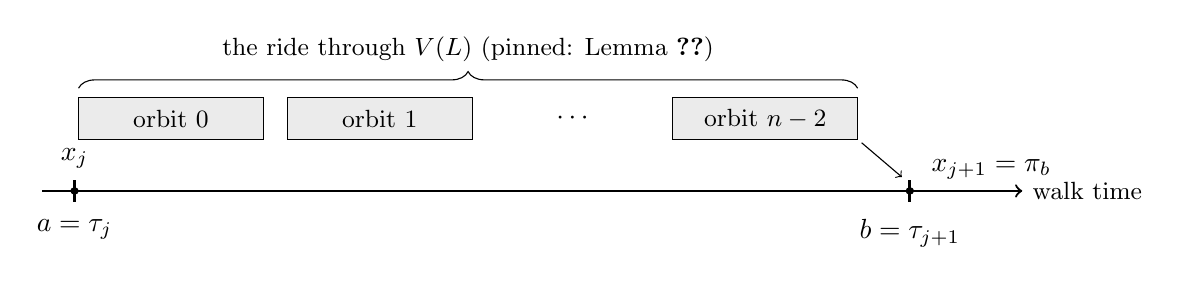
\begin{tikzpicture}[xscale=1.02,yscale=0.9]
  \draw[->,thick] (-0.4,0) -- (11.8,0) node[right] {\small walk time};
  \draw[very thick] (0,-0.15) -- (0,0.15);
  \node[below=3pt] at (0,-0.15) {\(a=\tau_j\)};
  \draw[very thick] (10.4,-0.15) -- (10.4,0.15);
  \node[below=3pt] at (10.4,-0.15) {\(b=\tau_{j+1}\)};
  \fill (0,0) circle (1.5pt);
  \fill (10.4,0) circle (1.5pt);
  \node[anchor=south] at (0,0.18) {\(x_j\)};
  \node[anchor=west] at (10.55,0.3) {\(x_{j+1}=\pi_b\)};
  \foreach \s/\e/\l in {0.05/2.35/{orbit \(0\)},2.65/4.95/{orbit \(1\)},7.45/9.75/{orbit \(n-2\)}}{
    \draw[fill=black!8] (\s,0.72) rectangle (\e,1.32);
    \node at ({(\s+\e)/2},1.02) {\small \l};
  }
  \node at (6.2,1.02) {\(\cdots\)};
  \draw[decorate,decoration={brace,amplitude=6pt}] (0.05,1.45) -- (9.75,1.45)
    node[midway,above=6pt] {\small the ride through \(V(L)\) (pinned: Lemma \ref{lem:pinned})};
  \draw[->,shorten >=3pt] (9.8,0.68) -- (10.38,0.12);
\end{tikzpicture}
\caption{A fresh switch-free \(L\)-window (Definition \ref{def:windowmodes}): the walk enters
\(L\) at \(x_j\), rides its rotation orbits in the canonical order, and leaves by the terminal
edge \(\pi_{b-1}\to\pi_b\) into the next first entry.  The window is \emph{full} when all
\(n-1\) orbits are completed (then \(\pi_{b-1}\) is the corner and Lemma \ref{lem:cornerexit}
classifies the exit), \emph{short} when it stops earlier (then, if the exit is not a weight-\(2\) door, a whole
orbit of \(V(L)\) is missed and Lemma \ref{lem:missed} traces its later first visit).}
\label{fig:window}
\end{figure}


\begin{lemma}[Local tight-edge classification]\label{lem:localtight}
Let \(\sigma=\pi_i\), \(z=\pi_{i+1}\), and \(w=\wt(\sigma,z)\).  Let
\[
  d_i=w-(\Delta p_i+\Delta c_i+\Delta v_i)
\]
be the local defect.  If \(d_i=0\), then \(w\le 3\).  More precisely:

\begin{enumerate}
\item If \(w=1\), then \(z=\rho(\sigma)\).  The edge stays in the same rotation orbit and
does not enter a new marked \(2\)-loop.
\item If \(w=2\), then
\[
  z=\sigma_3\sigma_4\cdots\sigma_n\sigma_2\sigma_1.
\]
The rotation orbit of \(\sigma\) is incident with the landing loop \(L(z)\).  If
\(\sigma\in V(L)\) for a marked \(2\)-loop \(L\), and \(L(z)=L\), then the edge is the standard
HPV door of \(L\), leading from the rotation orbit of \(\sigma\) to a different rotation orbit
of \(L\) (its successor in the canonical ride of Section 4).  If the target is not a first entry of a marked
\(2\)-loop, tightness forces
\[
  \Delta p_i=\Delta c_i=1,\qquad \Delta v_i=0.
\]
Thus this same-loop door can be tight only when \(\sigma\) completes its rotation orbit and
\(z\) is new.
\item If \(w=2\), \(\sigma\in V(L)\) for a marked \(2\)-loop \(L\), and \(L(z)\ne L\), then the rotation orbit of
\(\sigma\) is incident with both \(L\) and \(L(z)\).
\item If \(w=3\), then tightness forces
\[
  \Delta p_i=\Delta c_i=\Delta v_i=1.
\]
(The landing options of a tight weight-\(3\) exit at the end of a completed fresh ride are
classified in Lemma \ref{lem:cornerexit}.)
\end{enumerate}
\end{lemma}

\begin{proof}
Write
\[
  \sigma=s_1s_2\cdots s_n .
\]
If \(w=k\), then the defining overlap condition gives
\[
  z=s_{k+1}s_{k+2}\cdots s_n t_1\cdots t_k,
\]
where \(t_1,\ldots,t_k\) are the discarded symbols \(s_1,\ldots,s_k\) in some order.  Properness
means that no shorter prefix \(t_1\cdots t_h\), \(1\le h<k\), already produces a permutation
window; this is condition (prop) of Section 2:
\[
  \{t_1,\ldots,t_h\}\ne \{s_1,\ldots,s_h\}\qquad(1\le h<k).
\]

For any edge, each of \(\Delta p_i,\Delta c_i,\Delta v_i\) is either \(0\) or \(1\).  Hence
\(\Delta p_i+\Delta c_i+\Delta v_i\le3\), and \(d_i=0\) implies \(w\le3\).

If \(w=1\), then \(t_1=s_1\), so \(z=s_2\cdots s_ns_1=\rho(\sigma)\).  This is rotation inside
the same full rotation orbit.  It does not enter a new marked \(2\)-loop.

If \(w=2\), condition (prop) rules out \(t_1=s_1\).  Thus
\[
  (t_1,t_2)=(s_2,s_1),
\]
which gives the displayed weight-\(2\) door.  Deleting the last symbol of \(z\) gives
\[
  s_3s_4\cdots s_ns_2,
\]
which is cyclically equivalent to the word obtained from \(\sigma\) by deleting \(s_1\).  Hence
the full rotation orbit of \(\sigma\) is incident with \(L(z)\).  If \(\sigma\in V(L)\), it is
also incident with \(L\).

Now suppose this \(w=2\) edge is not a first entry of a marked \(2\)-loop.  Then \(\Delta v_i=0\).
Since \(d_i=0\),
\[
  2=\Delta p_i+\Delta c_i.
\]
Both summands are \(0\)-\(1\) valued, so \(\Delta p_i=\Delta c_i=1\).  Thus the edge visits a new
permutation and completes the source rotation orbit (Lemma \ref{lem:deltac}).  In particular, a
same-loop weight-\(2\) door is tight only when it is taken after finishing the source rotation
orbit; within a ride this is precisely the door to the following orbit of the ride.

If \(w=3\), then \(d_i=0\) gives
\[
  3=\Delta p_i+\Delta c_i+\Delta v_i.
\]
Again the increments are \(0\)-\(1\) valued, so all three increments equal \(1\).  The properness
condition (prop) leaves exactly the following three tails:
\[
\begin{array}{c|c}
(t_1,t_2,t_3) & z\\ \hline
(s_2,s_3,s_1) & s_4\cdots s_ns_2s_3s_1,\\
(s_3,s_1,s_2) & s_4\cdots s_ns_3s_1s_2,\\
(s_3,s_2,s_1) & s_4\cdots s_ns_3s_2s_1 .
\end{array}
\]
The table is recorded for later use: Lemma \ref{lem:cornerexit} classifies the three landings at
the end of a completed fresh ride.
\end{proof}

\begin{lemma}[Immediate charge cases]\label{lem:immediate}
Let \(j\in A_0\), and use the notation of Definition \ref{def:windowmodes}.  Write
\(\sigma=\pi_{b-1}\) and \(z=\pi_b=x_{j+1}\).  If any one of the following holds, then
\(\mathcal C(j)\ne\varnothing\):
\[
\begin{array}{ll}
\text{\rm (i)} & \wt(\sigma,z)=2,\\
\text{\rm (ii)}& \text{the \(L\)-window is not fresh},\\
\text{\rm (iii)}& \text{the \(L\)-window contains a switch}.
\end{array}
\]
\end{lemma}

\begin{proof}
Since \(j\in A_0\), every edge in \(a\le i<b\) has zero defect.  In particular the final edge
\(\sigma\to z\) is tight, and \(z\ne\rho(\sigma)\), because \(b\) is a first entry time.

For (i), the word form of a proper weight-\(2\) nonrotation edge (Lemma \ref{lem:localtight}) gives
\(\sigma\in V(L')\).  The source \(\sigma\) is visited at time \(b-1\), while \(L'\) is first
entered at time \(b\).  Thus \(L'\) is a pre-entry owner of the rotation orbit \(O\) of
\(\sigma\).  By Lemma \ref{lem:ownerbook}, \(O\in D\), \(L'\in\Omega(O)\), and \(L'\ne F(O)\).
Hence \((O,L')\in\mathcal C(j)\).

For (ii), choose \(t<a\) with \(\pi_t\in V(L)\), and let \(O\) be the rotation orbit of
\(\pi_t\).  Since \(L\) is first entered at time \(a\), the loop \(L\) is a pre-entry owner of
\(O\).  Lemma \ref{lem:ownerbook} gives \(O\in D\) and \(L\in\Omega(O)\), so
\((O,L)\in\mathcal C(j)\).

For (iii), let \(i\) be a switch and let \(O\) be the rotation orbit of \(\pi_i\).  The condition
\(\pi_i\in V(L)\) says \(L\in\Omega(O)\).  The word form of a weight-\(2\) door (Lemma \ref{lem:localtight}) gives
\(\pi_i\in V(L(\pi_{i+1}))\).  Since \(\operatorname{last}(\pi_{i+1})\ne \alpha\), the loop
\(L(\pi_{i+1})\) is not \(L\); it is activated by the nonrotation edge \(\pi_i\to\pi_{i+1}\).  Thus
\(O\) has two distinct entered owners, so \(O\in D\), and again \((O,L)\in\mathcal C(j)\).
\end{proof}

\begin{lemma}[Internal orbit-end alternatives]\label{lem:orbitendclass}
Let \(j\in A_0\), and use the notation of Definition \ref{def:windowmodes}.  Assume that the
\(L\)-window is fresh and switch-free.  Let \(i\) be an internal edge of this window:
\[
  a\le i,\qquad i+1<b.
\]
Suppose that \(\pi_i\in V(L)\) and that every vertex in the rotation orbit
\(O\) of \(\pi_i\) has appeared by time \(i\).  If \(d_i=0\), then \(O\) is not already counted by
\(c\) before the edge, and the edge is one of the following two forms:
\[
\begin{array}{ll}
\text{\rm (a)} & \pi_{i+1}=\rho(\pi_i),\text{ the closing rotation of }O,\\
\text{\rm (b)} & \pi_i\to\pi_{i+1}\text{ is the standard same-loop weight-\(2\) door in }L,
                  \text{ and }\pi_{i+1}\text{ is new.}
\end{array}
\]
After case \({\rm (a)}\), no further internal zero-defect edge can start from a vertex of \(O\).
\end{lemma}

\begin{proof}
The edge is internal to the interval between two consecutive first entries, so it first-enters no
marked \(2\)-loop and \(\Delta v_i=0\).  If \(O\) was already counted by \(c\) before the edge,
then \(\Delta c_i=0\): by Lemma \ref{lem:deltac} only the class of the source \(\pi_i\), which is
\(O\), could change status, and it is already counted.  Since every vertex of \(O\) has already
appeared, a weight-\(1\) rotation
has \(\Delta p_i=0\), hence positive defect.  A tight weight-\(2\) edge with \(\Delta v_i=0\)
would have \(\Delta p_i=\Delta c_i=1\) by Lemma \ref{lem:localtight}, impossible because
\(\Delta c_i=0\).  A tight edge of weight \(3\) would have \(\Delta v_i=1\), also impossible.
Thus \(O\) cannot already be counted.

Now \(O\) is not yet counted.  If \(d_i=0\) and \(\wt(\pi_i,\pi_{i+1})=1\), Lemma
\ref{lem:localtight} says the edge is the rotation \(\rho\), and since all vertices of \(O\) have
appeared, this is exactly the closing rotation that first counts \(O\).

If \(\wt(\pi_i,\pi_{i+1})=2\), Lemma \ref{lem:localtight} gives the proper weight-\(2\) door.  If
its landing loop is not \(L=(\alpha,K)\), then the landing marker is not \(\alpha\): with marker \(\alpha\), the
deleted word is cyclically equivalent to the deleted word of \(\pi_i\), and the landing loop would
be \(L\).  Thus a different landing loop is exactly a switch in the sense of Definition
\ref{def:windowmodes}, contrary to the switch-free hypothesis.  Hence it is the standard
same-loop door in \(L\).  Because the edge is internal, \(\Delta v_i=0\), and tightness gives
\(\Delta p_i=\Delta c_i=1\); in particular the target is new.

Finally, weight \(3\) cannot be tight on an internal edge, because Lemma \ref{lem:localtight}
would force \(\Delta v_i=1\).  After the closing rotation in case \({\rm (a)}\), the orbit \(O\)
has been counted by \(c\).  The first paragraph then rules out any later internal zero-defect edge
whose source lies in \(O\).
\end{proof}

\begin{lemma}[Anchored boundary edge]\label{lem:boundary}
Let \(L\) be an entered marked \(2\)-loop, and suppose that \(L\) was already entered before time
\(i\).  Let
\[
  \sigma=\pi_i,\qquad z=\pi_{i+1},
\]
and assume \(z\in V(L)\) and \(d_i=0\).  Suppose also that the edge
\(\sigma\to z\) is an anchored boundary into a later ride in \(L\): the active loop before the
edge is \(H_i=H\ne L\) (in particular the edge is not an interior same-loop door of a ride
already in \(L\), such a door having active loop \(L\)).
Then there is a shared rotation orbit \(O'\) with \(L\in\Omega(O')\).
\end{lemma}

\begin{proof}
By the definition of the active loop, \(\sigma\in V(H)\).
If \(\sigma\in V(L)\), then the rotation orbit of \(\sigma\) is incident with both \(L\) and
\(H\).  The two owners are distinct by hypothesis, so this orbit is shared and is owned by \(L\).

Assume now that \(\sigma\notin V(L)\).  Lemma \ref{lem:localtight} gives
\(\wt(\sigma,z)\le3\).  The weight cannot be \(1\), since \(V(L)\) is closed under rotation and
\(z=\rho(\sigma)\) would imply \(\sigma\in V(L)\).

If \(\wt(\sigma,z)=2\), Lemma \ref{lem:localtight} says that the rotation orbit of \(\sigma\)
is incident with \(L(z)\).  If \(L(z)=L\), rotation-closure of \(V(L)\) again gives
\(\sigma\in V(L)\), a contradiction.  Thus \(L(z)\ne L\).  This nonrotation edge activates
\(L(z)\), and the rotation orbit of \(z\) is incident with both \(L\) and \(L(z)\).  Hence
that orbit is shared and owned by \(L\).

Finally suppose \(\wt(\sigma,z)=3\).  Since \(d_i=0\), Lemma \ref{lem:localtight} gives
\(\Delta v_i=1\).  But \(L\) was already entered and \(z\in V(L)\).  Therefore the landing loop
generated by \(z\) cannot be \(L\); otherwise no new marked \(2\)-loop would be entered at this
edge.  Thus \(L(z)\ne L\).  The edge activates \(L(z)\), and again the rotation orbit of
\(z\) is incident with the two distinct entered loops \(L\) and \(L(z)\).
\end{proof}

\begin{lemma}[Pinned fresh window]\label{lem:pinned}
Let \(j\in A_0\), and use the notation of Definition \ref{def:windowmodes}.  Assume that the
\(L\)-window is fresh and switch-free.  Put \(N=b-a\) and \(x=x_j\).  Let
\[
  R_{h,r}\qquad(0\le h\le n-2,\ 0\le r<n)
\]
denote the HPV ride through \(L\) starting at \(x\): \(R_{h,0}\) is the first vertex of the
\(h\)-th rotation orbit of this ride, \(R_{h,r}=\rho^r(R_{h,0})\), and
\(R_{h+1,0}\) is the target of the standard weight-\(2\) door out of \(R_{h,n-1}\).
The indices \(h,r\) are zero-based offsets inside this displayed ride; walk times remain
one-based throughout.

Then the following pinning statement holds:
\[
  \pi_{a+o}=R_{\lfloor o/n\rfloor,\;o\bmod n} \tag{$\dagger$}
\]
whenever \(o<N-1\) and \(o<n(n-1)\).  In addition, if \(N-1\not\equiv 0\pmod n\) and
\(N\le n(n-1)\), then \((\dagger)\) also holds for \(o=N-1\).  Consequently:
\begin{enumerate}
\item If \(N=n(n-1)\), then
\[
  \{\pi_a,\pi_{a+1},\ldots,\pi_{b-1}\}=V(L),
\]
and \(\pi_{b-1}=R_{n-2,n-1}\).
\item If
\[
  (N-1)\equiv n-1\pmod n,\qquad N\le (n-2)n,
\]
then the full rotation orbit
\[
  \{R_{n-2,0},R_{n-2,1},\ldots,R_{n-2,n-1}\}\subseteq V(L)
\]
is missed by \(\pi_a,\ldots,\pi_{b-1}\).
\end{enumerate}
\end{lemma}

\begin{proof}
The pinning formula \((\dagger)\) is proved by induction over the rotation-orbit blocks.  We
maintain the following invariant:
at every pinned internal offset, the vertex lies in \(V(L)\) and the active loop is \(L\).  At
\(o=0\), this is \(\pi_a=x=R_{0,0}\), and \(L\) is first entered at time \(a\).  Suppose the walk
has been pinned through a vertex \(R_{h,r}\), put \(o=hn+r\), and assume that the next offset still
has to be pinned:
\[
  o+1<N-1,\qquad o+1<n(n-1).
\]
Since \(j\in A_0\), the next edge has zero defect.  Also, no marked \(2\)-loop is first entered at
an internal time \(a+1,\ldots,b-1\).

If \(r<n-1\), the current rotation orbit has not yet been completed.  A nonrotational edge of
weight \(2\) or \(3\) would have \(\Delta c=0\); because it is internal it also has
\(\Delta v=0\).  Lemma \ref{lem:localtight} then gives positive defect unless the edge is the
weight-\(1\) rotation.  Hence the next vertex is \(R_{h,r+1}\), and the active loop remains \(L\).

If \(r=n-1\), the source orbit has just been completed.  Since \(o+1<n(n-1)\), we have
\(h<n-2\).  Lemma \ref{lem:orbitendclass} says that a zero-defect internal edge is either the
standard same-loop door, whose new target is \(R_{h+1,0}\), or the closing rotation back into the
completed orbit.  The closing rotation cannot occur here: since \(o+1<N-1\), the offset
\(o+2\) still lies in the window, so the edge \emph{following} the closing rotation would be
internal and zero-defect with its source in the orbit \(O\) just counted by the closing
rotation --- exactly what the final sentence of Lemma \ref{lem:orbitendclass} forbids.  The
edge is therefore the standard same-loop door, and the next pinned vertex is \(R_{h+1,0}\).

The standard same-loop door activates \(L\) again, but since \(L\) is already entered it does not
increase \(v\); this is the sense in which a later nonrotation arrival differs from a first entry.
This proves \((\dagger)\) and the active-loop invariant for all offsets \(o<N-1\).  If
\(N-1\not\equiv 0\pmod n\), write
\(N-1=hn+r\) with \(0<r\le n-1\).  The block anchor \(R_{h,0}\) occurs at offset \(hn<N-1\)
unless \(h=0\), in which case it is \(x\).  The preceding rotation argument inside that block
pins the remaining \(r\) steps --- every source along the way has residue \(<n-1\) --- so
\((\dagger)\) also holds at the top offset \(N-1\).

If \(N=n(n-1)\), equation \((\dagger)\) lists exactly the \(n(n-1)\) vertices \(R_{h,r}\), with
\(0\le h\le n-2\) and \(0\le r<n\).  These are precisely \(V(L)\), and the last one is
\(R_{n-2,n-1}\).

For the second assertion, write \(N-1=hn+(n-1)\).  The inequality \(N\le(n-2)n\) gives
\(h\le n-3\).  By \((\dagger)\), every vertex \(\pi_a,\ldots,\pi_{b-1}\) lies in one of the rotation orbits
with index at most \(h\), so none lies in the last ride orbit
\(\{R_{n-2,r}:0\le r<n\}\).
\end{proof}

\begin{lemma}[No long non-door windows]\label{lem:nolong}
Let \(j\in A_0\), and use the notation of Definition \ref{def:windowmodes}.  Assume that the
\(L\)-window is fresh and switch-free.  If
\[
  \wt(\pi_{b-1},\pi_b)\ne2,
\]
then the window is not long:
\[
  b-a\le n(n-1).
\]
\end{lemma}

\begin{proof}
Put \(N=b-a\) and \(T=n(n-1)\).  Suppose, for contradiction, that \(N>T\).  Lemma
\ref{lem:pinned} pins the first \(T\) vertices of the window to the full ride through \(L\), so
\[
  \pi_{a+T-1}=R_{n-2,n-1}.
\]
The edge from \(\pi_{a+T-1}\) is internal and has zero defect.  At this source the last rotation
orbit of the ride has all its vertices present.  The standard same-loop door from
\(R_{n-2,n-1}\) returns to \(R_{0,0}=x_j\), already visited, so it cannot be the tight
same-loop-door alternative of Lemma \ref{lem:orbitendclass}.  Hence Lemma
\ref{lem:orbitendclass} leaves only the closing rotation to \(R_{n-2,0}\).  After that closing
rotation, the last rotation orbit has been counted by \(c\), and Lemma \ref{lem:orbitendclass}
rules out any further internal zero-defect edge starting from that orbit.  Therefore \(N=T+1\).

Now the terminal source \(\pi_{b-1}=\pi_{a+T}\) lies in that already counted last rotation orbit.
The terminal edge has zero defect, is not a rotation because \(b\) is a first-entry time, and is
not a weight-\(2\) edge by hypothesis.  Lemma \ref{lem:localtight} therefore forces it to have
weight \(3\) and \(\Delta c=1\).  But the only cyclic class whose counted status can change on
this edge is the source rotation orbit (Lemma \ref{lem:deltac}), and that orbit was already
counted on the preceding
closing rotation.  Thus \(\Delta c=0\), a contradiction.
\end{proof}

\begin{lemma}[Non-door short endings]\label{lem:orbitend}
Let \(j\in A_0\), and use the notation of Definition \ref{def:windowmodes}.  Assume that the
\(L\)-window is fresh, switch-free, and short.  If
\[
  \wt(\pi_{b-1},\pi_b)\ne2,
\]
then, with \(N=b-a\),
\[
  (N-1)\equiv n-1\pmod n,\qquad N\le(n-2)n.
\]
\end{lemma}

\begin{proof}
The terminal edge \(\pi_{b-1}\to\pi_b\) is zero-defect, because \(j\in A_0\).  It is not a
rotation, since \(b\) is a first-entry time for \(E_{j+1}\).  It is not a weight-\(2\) edge by
hypothesis, so Lemma \ref{lem:localtight} gives
\[
  \wt(\pi_{b-1},\pi_b)=3,\qquad
  \Delta p=\Delta c=\Delta v=1
\]
on this edge.  In particular the source rotation orbit is completed by the terminal edge.

We now show that the terminal source must be the last vertex of one of the ride orbits.  Suppose
first that \(N-1\equiv r\pmod n\) with \(0<r<n-1\).  The window is short, so \(N\le n(n-1)\),
and the \(o=N-1\) clause of Lemma \ref{lem:pinned} places \(\pi_{b-1}\) at the \(r\)-th rotation
of a ride orbit.  The later rotations of that same
orbit have not appeared in the fresh pinned window, and freshness excludes their occurrence before
time \(a\).  Hence the source rotation orbit is not complete, contradicting \(\Delta c=1\).

It remains to rule out \(N-1\equiv0\pmod n\).  If \(N=1\), the source is \(x\), and its rotation
orbit is plainly not complete.  If \(N>1\), write \(N-1=hn\) with \(h\ge1\); shortness gives
\(hn=N-1<n(n-1)\), so \(h\le n-2\).  The preceding internal edge starts at the pinned vertex
\(R_{h-1,n-1}\), the end of a ride orbit.  By Lemma \ref{lem:orbitendclass}, the preceding edge
is either the standard same-loop door or the closing rotation.  A standard same-loop door would
put \(\pi_{b-1}\) at \(R_{h,0}\), the first vertex of the next ride orbit (which exists, since
\(h\le n-2\)), again not complete.  A closing rotation would return to a rotation
orbit already counted as completed, so the terminal edge would have \(\Delta c=0\)
(Lemma \ref{lem:deltac}), not
\(\Delta c=1\).  Therefore neither case is possible, and we must have
\[
  N-1\equiv n-1\pmod n .
\]
Since the window is short, \(N<n(n-1)\).  Writing \(N-1=hn+(n-1)\), we get
\[
  N=(h+1)n<n(n-1),
\]
so \(h+1\le n-2\), and hence \(N\le(n-2)n\).
\end{proof}

\begin{lemma}[Full-corner exit]\label{lem:cornerexit}
Let \(j\in A_0\), and use the notation of Definition \ref{def:windowmodes}.  Assume that the
\(L\)-window is fresh, switch-free, and full.  If
\[
  x_{j+1}\ne M(x_j),\qquad \wt(\pi_{b-1},\pi_b)\ne2,
\]
then there is a vertex
\[
  y\in V(L)\cap V(E_{j+1})
\]
which is visited before time \(b\).
\end{lemma}

\begin{proof}
Write the entry permutation as \(x_j=u\alpha\), with \(\alpha\) the marker of \(L\).  Rotate
\(u\) by \(n-2\) places and write
\[
  u^{(n-2)}=\beta\,\gamma\,r.
\]
By Lemma \ref{lem:pinned}, the full fresh ride reaches the corner
\[
  \pi_{b-1}=\alpha\,\beta\,\gamma\,r .
\]
The terminal edge is zero-defect, is not a rotation because \(b\) is a first-entry time, and is
not a weight-\(2\) edge by hypothesis.  Hence Lemma \ref{lem:localtight} gives a proper
weight-\(3\) edge.  The three proper tails from the corner are
\[
\begin{array}{c|c}
\text{tail} & \text{landing vertex}\\ \hline
(\beta,\gamma,\alpha) & r\,\beta\,\gamma\,\alpha,\\
(\gamma,\alpha,\beta) & r\,\gamma\,\alpha\,\beta,\\
(\gamma,\beta,\alpha) & r\,\gamma\,\beta\,\alpha .
\end{array}
\]
The third landing vertex is \(M(x_j)\), so it is excluded by the break condition.  The first
landing vertex generates the same marked \(2\)-loop \(L\): deleting \(\alpha\) gives
\(r\beta\gamma\), cyclically equivalent to \(\beta\gamma r\).  Since \(L\) was already entered at
time \(a\), that landing cannot be the first entry \(E_{j+1}\).

Thus the landing vertex is \(r\gamma\alpha\beta\), and \(E_{j+1}=(\beta,[r\gamma\alpha])\).  Put
\[
  y=r\,\beta\,\gamma\,\alpha .
\]
Deleting \(\alpha\) from \(y\) gives \(r\beta\gamma\), cyclically equivalent to
\(\beta\gamma r\), so \(y\in V(L)\).  Deleting \(\beta\) from \(y\) gives \(r\gamma\alpha\), so
\(y\in V(E_{j+1})\).  The window is full, hence every vertex of \(V(L)\), including \(y\), was
visited before time \(b\).
\end{proof}

\begin{lemma}[Full residual charge]\label{lem:fullresidual}
Let \(j\in A_0\), and use the notation of Definition \ref{def:windowmodes}.  Assume the
\(L\)-window is fresh, switch-free, and full.  If
\[
  x_{j+1}\ne M(x_j),\qquad \wt(\pi_{b-1},\pi_b)\ne2,
\]
then \(\mathcal C(j)\ne\varnothing\).
\end{lemma}

\begin{proof}
By Lemma \ref{lem:cornerexit}, there is a vertex
\[
  y\in V(L)\cap V(L')
\]
visited before time \(b\), where \(L'=E_{j+1}\).
Because \(L'\) is first entered at time \(b\), \(L'\) is a pre-entry owner of the rotation orbit
\(O\) of \(y\).  Lemma \ref{lem:ownerbook} gives \(O\in D\) and \(L'\ne F(O)\), so
\((O,L')\in\mathcal C(j)\).
\end{proof}

\begin{lemma}[Anchored missed-orbit dichotomy]\label{lem:missed}
Let \(L\) be an entered marked \(2\)-loop, and let \(O\subseteq V(L)\) be a rotation orbit.
Suppose \(t\) is the first time at which the walk visits \(O\).  Suppose also that there is a
first-entry time \(t_0\le t\) such that \(L\) was already entered before time \(t_0\).  Then either
there is a shared rotation orbit \(O'\) with \(L\in\Omega(O')\), or there is an edge \(i\in P\) with
\[
  \pi_{i+1}\in V(L).
\]
\end{lemma}

\begin{proof}
If some edge \(\pi_i\to\pi_{i+1}\) with \(t_0\le i<t\) has positive defect and
\(\pi_{i+1}\in V(L)\), we are done.  We may therefore assume that every edge in this anchored
return segment whose target lies in \(V(L)\) has zero defect.

The entry into \(O\) cannot be a weight-\(1\) rotation, since then the preceding vertex would also
lie in \(O\), contradicting the minimality of \(t\).  Let \(H_t=L(\pi_t)\) be the landing marked
\(2\)-loop at the first visit to \(O\).  If \(H_t\ne L\), then \(O\) is owned by the two distinct
entered loops \(L\) and \(H_t\), so \(O\) is shared and we may take \(O'=O\).

It remains to consider \(H_t=L\).  The edge into \(O\) is then a return to the already entered loop
\(L\).  In particular \(t>t_0\): if \(t=t_0\), the first entry at time \(t_0\) would first-enter the
loop it activates, namely \(H_t=L\) --- but \(L\) was entered before \(t_0\).  For the same reason
\(t\) itself is not a first-entry time.

Let \(s\) be the last index before \(t\) at which the walk is anchored, meaning that \(s\) is a
first-entry time or \(\pi_s\notin V(L)\).  Such an \(s\) exists --- \(t_0\) itself is a
first-entry time, hence anchored, and \(t_0<t\) --- so \(t_0\le s<t\).  By maximality of
\(s\), every vertex \(\pi_{s+1},\ldots,\pi_{t-1}\) lies in \(V(L)\) and no index in
\(s+1,\ldots,t-1\) is a first-entry time; combined with \(\pi_t\in O\subseteq V(L)\) and the
previous paragraph, every vertex \(\pi_{s+1},\ldots,\pi_t\) lies in \(V(L)\), and there is no
first-entry time among \(s+1,\ldots,t\).  Thus the segment stays inside \(V(L)\), without first entering any new marked
\(2\)-loop, and ends at the first visit to \(O\).

Let \(H_s\) be the active loop at time \(s\).  It is entered, and the active-loop definition gives
\(\pi_s\in V(H_s)\).  Also \(H_s\ne L\).  If \(s\) is a first-entry time, then \(H_s=L(\pi_s)\); since
\(L\) had already been entered before \(t_0\le s\), the loop first entered at \(s\) is not \(L\).  If
\(s\) is not a first-entry time, then the definition of anchor gives \(\pi_s\notin V(L)\), whereas
\(\pi_s\in V(H_s)\).

An ordinary internal HPV door of a ride in \(L\) is, by definition, a weight-\(2\) same-loop door
whose source and target lie in \(V(L)\) and whose active loop before the edge is already \(L\).
The edges with \(s<i<t\) have this form when the same-loop door occurs.  The boundary edge
\(\pi_s\to\pi_{s+1}\) does not: its active loop before the edge is \(H_s\ne L\).  If this boundary
edge has positive defect, then it lands in \(V(L)\) and gives the second alternative.

Assume instead that the boundary edge has zero defect.  We check the hypotheses of Lemma
\ref{lem:boundary}.  The loop \(L\) was already entered before time \(t_0\), hence before time
\(s\).  The target \(\pi_{s+1}\) lies in \(V(L)\) by the choice of the last anchor \(s\).  The
active loop before the edge is \(H_s\ne L\), as proved above.  Thus Lemma
\ref{lem:boundary} applies, with previous loop \(H_s\),
and gives a shared rotation orbit \(O'\) with \(L\in\Omega(O')\), the first alternative.
\end{proof}

\begin{lemma}[Short residual dispatch]\label{lem:shortresidual}
Let \(j\in A_0\), and use the notation of Definition \ref{def:windowmodes}.  Assume the
\(L\)-window is fresh, switch-free, and short.  If \(\wt(\pi_{b-1},\pi_b)\ne2\), then either
\(\mathcal C(j)\ne\varnothing\), or there is an edge \(i\in P\) such that
\[
  \pi_{i+1}\in V(L).
\]
\end{lemma}

\begin{proof}
Put \(N=b-a\).  Lemma \ref{lem:orbitend} gives
\[
  (N-1)\equiv n-1\pmod n,\qquad N\le(n-2)n.
\]
Lemma \ref{lem:pinned} therefore gives a rotation orbit \(O\subseteq V(L)\) missed by
\(\pi_a,\ldots,\pi_{b-1}\).  Freshness says no vertex of \(V(L)\), hence no vertex of \(O\), occurs
before time \(a\).  Since \(W\) is covering, let \(t\) be the first time at which the walk visits
\(O\).  Then \(t\ge b\).

Apply Lemma \ref{lem:missed} with the anchor \(t_0=b\).  The loop \(L\) was entered at time
\(a<b\), while \(b\) is the first entry time of \(E_{j+1}\), so this is an anchored return to an
already entered loop.  If Lemma \ref{lem:missed} gives an edge \(i\in P\) with
\(\pi_{i+1}\in V(L)\), we have the crossing alternative.  Otherwise it gives a shared orbit
\(O'\) with \(L\in\Omega(O')\).  Since \(L=E_j\), the pair \((O',L)\) lies in \(\mathcal C(j)\).
\end{proof}

\begin{lemma}[Endpoint-or-cross dispatch]\label{lem:dispatch}
For every \(j\in A_0\), either \(\mathcal C(j)\ne\varnothing\), or there is an edge
\(i\in P\) such that
\[
  \pi_{i+1}\in V(E_j).
\]
\end{lemma}

\begin{proof}
Fix \(j\in A_0\), and use the notation of Definition \ref{def:windowmodes}.  Write
\(\sigma=\pi_{b-1}\) and \(z=\pi_b\).  If \(\wt(\sigma,z)=2\), Lemma \ref{lem:immediate} gives a
charge.  Assume \(\wt(\sigma,z)\ne2\).

If the \(L\)-window is not fresh, Lemma \ref{lem:immediate} gives a charge.  If it is fresh but
contains a switch, the same lemma again gives a charge.  We are left with a fresh switch-free
window.  Lemma \ref{lem:nolong} excludes the long case under the standing non-door hypothesis.
Since \(j\in A_0\subseteq A\), we have \(x_{j+1}\ne M(x_j)\).  If it is full, Lemma
\ref{lem:fullresidual} gives a charge.  Otherwise it is short, and Lemma \ref{lem:shortresidual}
gives either a charge or an edge \(i\in P\) with \(\pi_{i+1}\in V(L)=V(E_j)\).
\end{proof}

Let \(G\subseteq A_0\) be the charged breaks and \(B=A_0\setminus G\).

\begin{lemma}[Uncharged breaks]\label{lem:uncharged}
\[
  |B|\le n|P|. \tag{8}
\]
\end{lemma}

\begin{proof}
For each \(j\in B\), Lemma \ref{lem:dispatch} provides at least one positive-defect edge whose
target lies in \(V(E_j)\); choose one such witnessing edge and call it \(i(j)\in P\).  For a
fixed \(i\), at most \(n\) entered marked \(2\)-loops \(L\) satisfy
\(\pi_{i+1}\in V(L)\): the marker \(\alpha\) of \(L=(\alpha,K)\) can be chosen in \(n\) ways, and once \(\alpha\)
is fixed the cyclic class \(K\) is forced to be
\([\operatorname{del}_\alpha(\pi_{i+1})]\).  The map \(j\mapsto E_j\) is injective, since the \(E_j\) are
first entries of distinct marked \(2\)-loops.  Hence the assignment \(j\mapsto(i(j),E_j)\) injects
\(B\) into a set of size at most \(n|P|\).
\end{proof}

An incident slot
is a pair \((O,L)\) with \(O\in D\) and \(O\) incident with the entered marked \(2\)-loop \(L\).
The slot is noninitial if
\(L\ne F(O)\).  For an incident slot \((O,L)\), put
\[
  G_{O,L}=\{j\in G:O(j)=O,\ L(j)=L\}.
\]

\begin{lemma}[Slot fibers]\label{lem:slot}
For every incident slot \((O,L)\), \(|G_{O,L}|\le 2\).  If \(L=F(O)\), then
\(|G_{O,L}|\le 1\).  If \(|G_{O,L}|=2\), then one of the two charges is left and the other is
right.
\end{lemma}

\begin{proof}
Split \(G_{O,L}\) into left and right charges.  If two left charges existed, then
\[
  L=E_j=E_{j'}
\]
for two distinct first-entry indices \(j\ne j'\), contradicting the fact that the \(E_t\) are listed
without repetition.  Thus there is at most one left charge.  The same argument applied to
\[
  L=E_{j+1}=E_{j'+1}
\]
shows that there is at most one right charge.  Hence \(|G_{O,L}|\le 2\).  By construction, right
charges are never assigned to the initial slot \(F(O)\), so an initial slot receives at most the one
possible left charge.  If a slot receives two charges, the preceding left/right bounds force one of
each type.
\end{proof}

Let \(C\) be the number of noninitial slots with \(|G_{O,L}|=2\).  Since there are
\(\mu(O)-1\) noninitial slots over \(O\),
\[
  C\le \sum_{O\in D}(\mu(O)-1)=q. \tag{9}
\]

\begin{lemma}[Refined break count]\label{lem:fiber}
\[
  |A_0|\le q+|D|+C+n|P|. \tag{10}
\]
\end{lemma}

\begin{proof}
By Lemma \ref{lem:uncharged}, it is enough to count \(G\).  Over a fixed shared orbit \(O\), Lemma
\ref{lem:slot} gives at most one charge to the initial slot, at most one charge to each of the
\(\mu(O)-1\) noninitial slots, and one additional charge for each double-charged noninitial slot.
Thus the number of charged breaks over \(O\) is at most
\[
  1+(\mu(O)-1)+C_O=\mu(O)+C_O,
\]
where \(C_O\) is the number of double-charged noninitial slots over \(O\).  Summing over
\(O\in D\),
\[
  |G|\le |D|+\sum_{O\in D}(\mu(O)-1)+C=|D|+q+C.
\]
Adding \(|B|\le n|P|\) proves the claim.
\end{proof}

\begin{lemma}[Short-block credit]\label{lem:short}
\[
  v(W)+C(n-3)\le (|A|+1)(n-2). \tag{11}
\]
\end{lemma}

\begin{proof}
By Lemma \ref{lem:slot}, a double-charged noninitial slot \((O,L)\) has one left charge and one
right charge.  Say the right charge occurs at break \(j\), so \(L=E_{j+1}\), and the left charge
occurs at break \(i\), so \(L=E_i\).  Since the \(E_t\) are distinct, \(i=j+1\).  Thus \(j\) and
\(j+1\) are consecutive breaks, and the block between them consists only of \(E_{j+1}\).  This block
has length \(1\), whereas the general block bound allowed length \(n-2\), so it saves \(n-3\).

Assign the slot \((O,L)\) to the right-charged break \(j\).  This assignment is injective: the break
\(j\) determines its chosen charge \((O(j),L(j))=(O,L)\).  Hence the \(C\) double-charged slots give
\(C\) distinct short blocks.  Adding these \(C(n-3)\) savings to the basic block bound (3) gives
the result.
\end{proof}

Proposition \ref{prop:twoparam} below consumes the walk only through the seven facts (4),
(5), (6a), (6b), (9), (10), and (11), read as constraints on the nine statistics
\(e,\ell,|P|,|A|,|A_0|,q,|D|,C,v\).  The coefficient-two bound is optimal for this
aggregate inequality system:

\begin{proposition}[Sharpness of the accounting interface]\label{prop:interface}
For every \(n\ge5\) and all nonnegative integers \(e,\ell\), the assignment
\begin{gather*}
  |P|=e,\qquad q=|D|=C=\ell(n-1),\qquad
  |A_0|=3\ell(n-1)+ne,\qquad |A|=3\ell(n-1)+(n+1)e,\\
  v=\bigl(2\ell(n-1)+(n+1)e+1\bigr)(n-2)+\ell(n-1)
\end{gather*}
of nonnegative integers satisfies all seven constraints, each with equality (an integral
certificate, not merely a real one).  Consequently the
system (4), (5), (6a), (6b), (9), (10), (11) does not imply, for any \(e,\ell\), any upper
bound on \(v\) smaller than \(\bigl(2\ell(n-1)+(n+1)e+1\bigr)(n-2)+\ell(n-1)\): every
conclusion derivable from these facts alone is consistent with the displayed values.
\end{proposition}

\begin{proof}
Facts (4), (6a), (6b), and (9) hold at once, and \(|A|=|A_0|+|P|\) gives (5).  For (10),
\(q+|D|+C+n|P|=3\ell(n-1)+ne=|A_0|\).  For (11),
\[
  \bigl(|A|+1\bigr)(n-2)-\bigl(2\ell(n-1)+(n+1)e+1\bigr)(n-2)
  \ =\ \ell(n-1)(n-2)\ =\ \ell(n-1)+\ell(n-1)(n-3),
\]
so \(v+C(n-3)=(|A|+1)(n-2)\) exactly.
\end{proof}

Any further improvement of the coefficient must therefore add a new structural fact about
covering walks, beyond the aggregate system (4)--(11); no better arrangement of the present
facts can supply it.

\section{The coefficient-two estimate}

\begin{proposition}\label{prop:twoparam}
Let \(n\ge 5\).  There is no covering walk \(W\) with
\[
  e(W)=e,\qquad v(W)=(n-2)!+\ell
\]
if
\[
  \bigl(2\ell(n-1)+(n+1)e+1\bigr)(n-2)+\ell(n-1)<(n-2)!+\ell . \tag{12}
\]
\end{proposition}

\begin{proof}
By (4), (5), (6a), (6b), and Lemma \ref{lem:fiber},
\[
\begin{aligned}
  |A|
    &\le |A_0|+|P|\\
    &\le q+|D|+C+n|P|+|P|\\
    &\le 2\ell(n-1)+C+(n+1)e .
\end{aligned}
\]
Using Lemma \ref{lem:short},
\[
\begin{aligned}
  (n-2)!+\ell+C(n-3)
    &=v(W)+C(n-3)\\
    &\le (|A|+1)(n-2)\\
    &\le \bigl(2\ell(n-1)+C+(n+1)e+1\bigr)(n-2).
\end{aligned}
\]
Therefore
\[
  (n-2)!+\ell
    \le \bigl(2\ell(n-1)+(n+1)e+1\bigr)(n-2)+C.
\]
Finally \(C\le q=\ell(n-1)\) by (9) and (6a), contradicting (12).
\end{proof}

\begin{lemma}\label{lem:corner}
Let \(n\ge 5\), and suppose
\[
  \bigl(2k(n-1)+1\bigr)(n-2)+k(n-1)<(n-2)!+k . \tag{13}
\]
If \(e,\ell\ge 0\) and \(e+\ell\le k\), then
\[
  \bigl(2\ell(n-1)+(n+1)e+1\bigr)(n-2)+\ell(n-1)<(n-2)!+\ell .
\]
\end{lemma}

\begin{proof}
Put \(\nu=n-2\).  Since \(n\ge 5\), \(\nu\ge 3\).  Define
\[
  P_k=\bigl(2k(\nu+1)+1\bigr)\nu+k(\nu+1)
\]
and
\[
  Q_{e,\ell}=\bigl(2\ell(\nu+1)+(\nu+3)e+1\bigr)\nu+\ell(\nu+1).
\]
A direct calculation gives
\[
  P_k+\ell-Q_{e,\ell}-k
    =\nu\bigl(e\nu+(k-e-\ell)(2\nu+3)\bigr)\ge 0.
\]
Thus \(Q_{e,\ell}+k\le P_k+\ell\).  Combining this with (13) gives
\[
  Q_{e,\ell}+k<(n-2)!+k+\ell,
\]
and the result follows.
\end{proof}

\begin{theorem}[Coefficient-two criterion]\label{thm:criterion}
Let \(n\ge 5\).  If \(k\ge 0\) satisfies
\[
  \bigl(2k(n-1)+1\bigr)(n-2)+k(n-1)<(n-2)!+k,
\]
then
\[
  \Lambda(n)\ge \HPV(n)+k+1.
\]
\end{theorem}

\begin{proof}
Suppose not, and choose a covering walk \(W\) with \(\len(W)\le \HPV(n)+k\).  By (2),
\[
  e(W)+r(W)+\ell(W)\le k,
\]
so \(e(W)+\ell(W)\le k\).  Lemma \ref{lem:corner} gives the two-parameter inequality (12) for
\(e=e(W)\) and \(\ell=\ell(W)\), contradicting Proposition \ref{prop:twoparam}.
\end{proof}

The criterion is linear in \(k\), so it can be solved once and for all.

\begin{lemma}[Solving the criterion]\label{lem:solve}
Let \(n\ge5\) and \(k\ge0\).  The criterion inequality
\((2k(n-1)+1)(n-2)+k(n-1)<(n-2)!+k\) holds if and only if
\[
  k(2n-1)\ <\ (n-3)!-1,
  \qquad\text{equivalently}\qquad
  k\ <\ \Bigl\lceil\frac{(n-3)!-1}{2n-1}\Bigr\rceil .
\]
\end{lemma}

\begin{proof}
The left side of the criterion is \(2k(n-1)(n-2)+(n-2)+k(n-1)\), and
\[
  2k(n-1)(n-2)+k(n-1)-k \ =\ k\bigl(2(n-1)(n-2)+(n-2)\bigr)\ =\ k(n-2)(2n-1),
\]
so, subtracting \(k\) from each side of the criterion and factoring, the criterion is
equivalent to
\[
  (n-2)\bigl(k(2n-1)+1\bigr)\ <\ (n-2)\cdot(n-3)!
\]
(using \((n-2)!=(n-2)\cdot(n-3)!\)), i.e.\ to \(k(2n-1)+1<(n-3)!\), i.e.\ to
\(k(2n-1)<(n-3)!-1\).  For an integer \(k\) and positive \(2n-1\), this says exactly
\(k<\lceil((n-3)!-1)/(2n-1)\rceil\).
\end{proof}

\begin{theorem}[The criterion, solved]\label{thm:solved}
For all \(n\ge 5\),
\[
  \Lambda(n)\ \ge\ \HPV(n)+\Bigl\lceil\frac{(n-3)!-1}{2n-1}\Bigr\rceil,
  \qquad\text{hence}\qquad
  S(n)\ \ge\ \HPV(n)+\Bigl\lceil\frac{(n-3)!-1}{2n-1}\Bigr\rceil .
\]
Moreover the ceiling is exact for the criterion: by Lemma \ref{lem:solve} the criterion fails at
\(k=\lceil((n-3)!-1)/(2n-1)\rceil\), so no larger bound is an instance of Theorem
\ref{thm:criterion}.
\end{theorem}

\begin{proof}
Put \(\kappa=\lceil((n-3)!-1)/(2n-1)\rceil\).  Since \(n\ge5\), \((n-3)!-1\ge1>0\), so
\(\kappa\ge1\), and \(k=\kappa-1\) satisfies \(k<\kappa\), hence the criterion by Lemma
\ref{lem:solve}.  Theorem \ref{thm:criterion} gives
\(\Lambda(n)\ge\HPV(n)+(\kappa-1)+1=\HPV(n)+\kappa\).  The word form follows from
\(\Lambda(n)\le S(n)\) (Section 2).
\end{proof}

\begin{corollary}[Point values]\label{cor:pointvalues}
\begin{gather*}
  \Lambda(5)\ge\HPV(5)+1,\qquad
  \Lambda(6)\ge\HPV(6)+1,\qquad
  \Lambda(7)\ge\HPV(7)+2,\qquad
  \Lambda(8)\ge\HPV(8)+8,\\
  \Lambda(9)\ge\HPV(9)+43,\qquad
  \Lambda(10)\ge\HPV(10)+266,\qquad
  \Lambda(11)\ge\HPV(11)+1920.
\end{gather*}
\end{corollary}

\begin{proof}
Apply Theorem \ref{thm:criterion} with \(k=0,0,1,7,42,265,1919\) respectively.  The criterion
\((2k(n-1)+1)(n-2)+k(n-1)<(n-2)!+k\), whose left side equals \((n-1)(2n-3)k+(n-2)\), reads
\[
\begin{array}{c|c|c}
n & \text{left side} & \text{right side}\\ \hline
5,\ k=0 & 28\cdot0+3=3 & 6+0=6\\
6,\ k=0 & 45\cdot0+4=4 & 24+0=24\\
7,\ k=1 & 66\cdot1+5=71 & 120+1=121\\
8,\ k=7 & 91\cdot7+6=643 & 720+7=727\\
9,\ k=42 & 120\cdot42+7=5047 & 5040+42=5082\\
10,\ k=265 & 153\cdot265+8=40553 & 40320+265=40585\\
11,\ k=1919 & 190\cdot1919+9=364619 & 362880+1919=364799
\end{array}
\]
and each row holds.  (In each case \(k\) is the largest admissible value.)  Equivalently, by
Theorem \ref{thm:solved}, the seven increments are the evaluations
\[
  \Bigl\lceil\tfrac{1}{9}\Bigr\rceil,\
  \Bigl\lceil\tfrac{5}{11}\Bigr\rceil,\
  \Bigl\lceil\tfrac{23}{13}\Bigr\rceil,\
  \Bigl\lceil\tfrac{119}{15}\Bigr\rceil,\
  \Bigl\lceil\tfrac{719}{17}\Bigr\rceil,\
  \Bigl\lceil\tfrac{5039}{19}\Bigr\rceil,\
  \Bigl\lceil\tfrac{40319}{21}\Bigr\rceil
  \ =\ 1,\ 1,\ 2,\ 8,\ 43,\ 266,\ 1920.
\]
\end{proof}

\section{The closed form}

By Theorem \ref{thm:solved} the exact bound of the criterion is the ceiling
\(\lceil((n-3)!-1)/(2n-1)\rceil\); this section records a single weaker but more
memorable factorial form, uniform over the theorem's whole range \(n\ge5\), with an
elementary certificate.

\begin{lemma}\label{lem:third}
For all \(n\ge 5\),
\[
  \Bigl\lceil\frac{(n-4)!}{3}\Bigr\rceil\ \le\
  \Bigl\lceil\frac{(n-3)!-1}{2n-1}\Bigr\rceil, \tag{14}
\]
with equality at \(n=5,6,7,8\), where both sides are \(1,1,2,8\).
\end{lemma}

\begin{proof}
For \(5\le n\le 8\) both sides evaluate to \(1,1,2,8\): the left sides are the
ceilings of \(\tfrac13,\tfrac23,\tfrac63,\tfrac{24}{3}\), the right sides the ceilings
of \(\tfrac19,\tfrac{5}{11},\tfrac{23}{13},\tfrac{119}{15}\).
For \(n\ge 9\), since the ceiling is monotone it suffices that
\[
  \frac{(n-4)!}{3}\ \le\ \frac{(n-3)!-1}{2n-1},
\]
i.e.\ \((2n-1)(n-4)!\le 3(n-3)!-3\).  Writing \((n-3)!=(n-3)(n-4)!\), this reads
\[
  (n-4)!\bigl(3(n-3)-(2n-1)\bigr)\ =\ (n-4)!\,(n-8)\ \ge\ 3,
\]
which holds because \(n-8\ge1\) and \((n-4)!\ge 5!=120\).
\end{proof}

\begin{corollary}[Uniform factorial form]\label{cor:third}
For all \(n\ge 5\),
\begin{gather*}
  \Lambda(n)\ \ge\ \HPV(n)+\Bigl\lceil\frac{(n-4)!}{3}\Bigr\rceil,
  \qquad\text{and hence}\\
  S(n)\ \ge\ n!+(n-1)!+(n-2)!+n-3+\Bigl\lceil\frac{(n-4)!}{3}\Bigr\rceil .
\end{gather*}
\end{corollary}

\begin{proof}
Combine Theorem \ref{thm:solved} with Lemma \ref{lem:third}; the word form follows from
\(\Lambda(n)\le S(n)\) (Section 2).
\end{proof}

\begin{corollary}\label{cor:words}
The reduction \(\Lambda(n)\le S(n)\) of Section 2 likewise transfers Theorem
\ref{thm:criterion} and Corollary \ref{cor:pointvalues} verbatim to \(S(n)\); in
particular \(S(5)\ge\HPV(5)+1=153\)
(the known exact value), \(S(6)\ge\HPV(6)+1=868\), \(S(7)\ge\HPV(7)+2=5886\), \(S(8)\ge\HPV(8)+8=46093\),
\(S(9)\ge\HPV(9)+43=408289\), \(S(10)\ge\HPV(10)+266=4032273\), and
\(S(11)\ge\HPV(11)+1920=43910408\).
\end{corollary}

\begin{remark}[The coefficient cannot reach one half]\label{rem:half}
For every \(n\ge 7\),
\[
  2\,\Bigl\lceil\frac{(n-3)!-1}{2n-1}\Bigr\rceil\ <\ (n-4)! . \tag{15}
\]
Indeed \(\lceil((n-3)!-1)/(2n-1)\rceil\le((n-3)!+2n-3)/(2n-1)\), and
\(2(n-3)!+4n-6<(2n-1)(n-4)!\) reduces, via \((n-3)!=(n-3)(n-4)!\), to
\(5\,(n-4)!>4n-6\), which holds from \(n=7\) on.  Thus no bound of the form
\(S(n)\ge\HPV(n)+c\,(n-4)!\) with a constant \(c\ge\tfrac12\) is available from the
criterion at any \(n\ge7\), while Corollary \ref{cor:third} attains \(c=\tfrac13\)
uniformly from \(n=5\).
\end{remark}

\section*{Provenance and acknowledgements}

This is an AI-derived result.  The mathematical content of this paper --- the
coefficient-two criterion, its proof, and the closed forms --- was produced by
large-language-model AI systems working in an extended iterative research loop.  The author
directed the research programme, set its goals and guardrails, and reviewed the results; the
proofs themselves were found by the AI systems.

\begin{thebibliography}{99}

\bibitem{AT}
D.~Ashlock and J.~Tillotson,
\emph{Construction of small superpermutations and minimal injective superstrings},
Congressus Numerantium \textbf{93} (1993), 91--98.

\bibitem{Egan}
G.~Egan,
\emph{Superpermutations},
web essay, October 2018 (updated).
\url{https://www.gregegan.net/SCIENCE/Superpermutations/Superpermutations.html}.
Accessed July 2026.

\bibitem{EV}
M.~Engen and V.~Vatter,
\emph{Containing all permutations},
Amer. Math. Monthly \textbf{128} (2021), 4--24.
Also arXiv:1810.08252.

\bibitem{Houston}
R.~Houston,
\emph{Tackling the minimal superpermutation problem},
arXiv:1408.5108 (2014).

\bibitem{HPV}
Anonymous 4chan Poster, Robin Houston, Jay Pantone, and Vince Vatter,
\emph{A lower bound on the length of the shortest superpattern}, October 25, 2018.
Available at \url{https://oeis.org/A180632/a180632.pdf}.
Accessed July 2026.

\bibitem{J2013}
N.~Johnston,
\emph{Non-uniqueness of minimal superpermutations},
Discrete Math. \textbf{313} (2013), 1553--1557.
Also arXiv:1303.4150.

\bibitem{JohnstonBlog}
N.~Johnston,
\emph{All minimal superpermutations on five symbols have been found},
blog post, August 13, 2014, reporting B.~Chaffin's verification of \(S(5)=153\).
Accessed July 2026:
\url{https://njohnston.ca/2014/08/all-minimal-superpermutations-on-five-symbols-have-been-found/}.

\bibitem{OEIS}
The On-Line Encyclopedia of Integer Sequences,
entry A180632 (\emph{minimal number of characters in a string containing every permutation of
\(n\) symbols as substrings}).
\url{https://oeis.org/A180632}.
Accessed July 2026.

\end{thebibliography}

\end{document}
